\chapter{Interacción Débil}\label{cap:weak_int}
El origen de cada interacción fundamental se debe a causas diferentes. Por un lado, la existencia de carga eléctrica produce fuerzas electromagnéticas en las partículas y las hace interactuar entre sí, mientras que la interacción fuerte se debe a la propiedad del color, mencionada en el capítulo anterior. No todas las partículas tienen carga ni color simultáneamente por lo que no todas son susceptibles a las mismas interacciones. El caso de la interacción débil es bastante interesante porque muchas partículas con propiedades distintas son sensibles a ella. Por ejemplo, los leptones no tienen carga de color, no ``sienten'' la interacción fuerte, mientras los neutrinos no tienen carga eléctrica, por lo que no pueden interactuar mediante fuerzas electromagnéticas. Sin embargo, ambos tipos de partículas pueden estar presentes en interacciones débiles.\cite{Griffiths2008} Además, la causa de la interacción débil, aunque no tiene un nombre específico, suele denotarse como \textit{carga débil}.

Los mesones $\PK$ y muchas otras partículas decaen por interacción débil. Desde el principio se consideró un tratamiento cuántico-relativista para describir la fuerza débil y muchos científicos han contribuido al desarrollo de su formalismo. Cada interacción ocurre gracias al intercambio de una partícula mediadora o portadora de la fuerza de interacción. En la interacción fuerte es el gluón y en la electromagnética es el fotón. Las partículas mediadoras encargadas de transmitir la fuerza débil entre los quarks y leptones son los bosones vectoriales, llamados así por tener espín 1. Estos bosones, de gran masa, portadores de la interacción débil pueden estar cargados eléctricamente $\PWpm$ o ser neutros $\PZzero$. 

Hasta la década de los 70, sólo se habían observado procesos de intercambio de bosones cargados $\PWpm$. En los años 60 se empezó a formular una teoría que aunaba la interacción débil junto con la electromagnética, conocida hoy en día como \textit{Teoría Electrodébil}. Esta teoría predecía la existencia del bosón neutro mediador de la fuerza débil y dicha hipótesis fue confirmada experimentalmente en 1973 \cite{BrianM}, con el hallazgo de $\PZzero$.

Este capítulo se centra, principalmente, en la descripción de procesos de interacción débil con intercambio de bosones $\PWpm$ o procesos de in\textit{teracción débil de corriente cargada} y nos servirá como base para el estudio del decaimiento de mesones $\PK$ cargados.

\section{Formalismo de la Interacción Débil}\label{cap:formalism}
Del mismo modo, las interacciones se describen mediante unas constantes, denominadas \textit{contantes de acoplamiento}, y productos entre los campos cuánticos de las partículas que intervienen en el proceso. Como $\mathcal{L}$ debe ser un escalar, sólo se permiten combinaciones entre campos que resulten en invariantes de Lorentz \cite{notas2020}. Esto es posible, ya que la TCC, entiende las interacciones como un intercambio de partículas mediadoras, tal y como se mencionó anteriormente. En su libro \cite{Bettini}, Bettini lo explica con el siguiente ejemplo: se tiene una partícula $a$ que interactúa en el campo mediado por el bosón $V$; en el vacío, $a$ está continuamente emitiendo y absorbiendo este bosón, tal y como se muestra en \ref{fig:bettini1}. No obstante, si una partícula $b$ se encuentra cerca de $a$ y tiene su misma interacción, puede absorber un bosón $V$ que previamente haya sido emitido por $a$ (ver \ref{fig:bettini2}). Entonces, se puede afirmar que $a$ y $b$ interactúan entre sí intercambiando un bosón $V$, es decir, combinando sus campos cuánticos.
\begin{figure}[h]
\begin{subfigure}{.5\textwidth}
  \centering
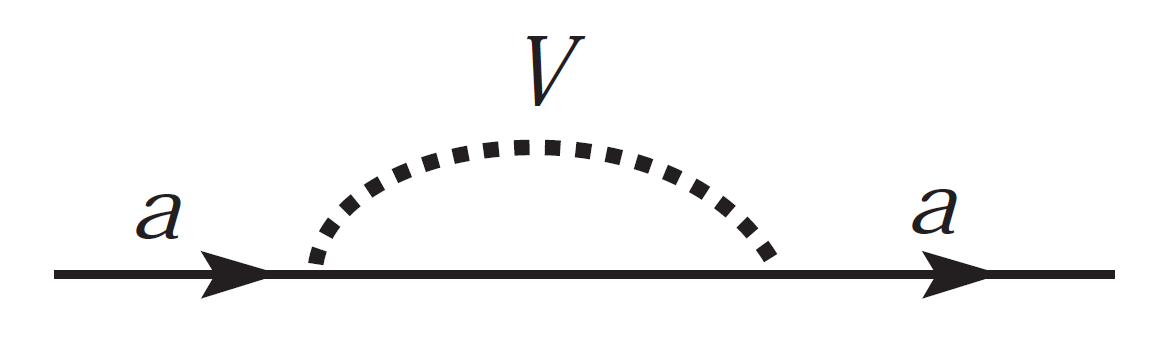
\includegraphics[width=0.6\linewidth]{{C:/Users/Carmen/Desktop/Universidad/TFG/Borradores/img/bettini1.PNG}}
\caption{$V$ emitido y reabsorbido por $a$}
  \label{fig:bettini1}
\end{subfigure}%
\begin{subfigure}{.5\textwidth}
  \centering
  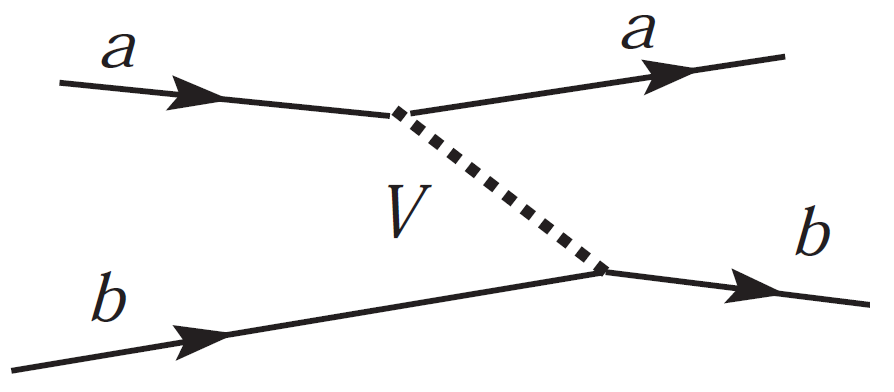
\includegraphics[width=0.6\linewidth]{{C:/Users/Carmen/Desktop/Universidad/TFG/Borradores/img/bettini2.PNG}}
  \caption{$V$ emitido por $a$ y absorbido por $b$}
  \label{fig:bettini2}
\end{subfigure}
\caption[Esquematización del proceso de interacción en TCC]{Proceso de interacción mediante intercambio del bosón mediador.  \cite{Bettini}}
\label{fig:bettini}
\end{figure}

Continuando con el ejemplo anterior, Bettini indica que el bosón mediador $V$ tiene, en general, una masa $m$ no nula, lo que provoca que, durante su emisión, se viole momentáneamente la conservación de energía $\Delta E = m$. Lo mismo, pero de forma opuesta ocurre durante su absorción. Así pues, la violación neta dura un $\Delta t$ y satisface la \textit{Relación de Indeterminación tiempo-energía}: $\Delta E \Delta t \leq \hbar$, lo que implica que $V$ sólo puede alejarse una distancia finita $R=c\Delta t$. Esta distancia equivale al rango de la fuerza de interacción, por lo tanto, cuanta mayor masa tenga el bosón mediador de una interacción, menor será su rango de alcance \cite{Bettini}. Dado que los bosones mediadores $\PWpm$ y $\PZzero$ tienen una masa muy grande ($m_W = \SI{80,379 \pm 0,012}{\GeV}$ GeV y $m_Z = \SI{91,1876 \pm 0,0021}{\GeV}$, respectivamente \cite{Zyla}), la fuerza débil tiene un alcance muy corto, más que cualquier otra interacción fundamental, resultando en una intensidad muy tenue; de ahí la denominación de `` interacción débil''.


\subsection{Interacción débil en el Modelo de Quarks}\label{sec:weak_int_quarks}
En el modelo de Quarks, la interacción débil se describe mediante Diagramas de Feynman, donde se produce un cambio de sabor en los quarks, emitiendo bosones $\PWpm$. Como consecuencia de la conservación del número leptónico en esta interacción, el acoplamiento de $\PWpm$ ocurre de manera estricta entre leptones de la misma generación \cite{Griffiths2008}: 
\begin{align}
\begingroup 
\renewcommand*{\arraystretch}{0.8}
\setlength\arraycolsep{10pt}
\begin{pmatrix} \nu _{e} \\ e \end{pmatrix} \qquad
\begin{pmatrix} \nu_{\mu } \\ \mu \end{pmatrix} \qquad
\begin{pmatrix} \nu_{\tau} \\ \tau \end{pmatrix}
\endgroup
\end{align}
No obstante, $W^{\pm}$ sí puede acoplarse a quarks de distintas generaciones:
\begin{align}
\begingroup 
\renewcommand*{\arraystretch}{0.8}
\setlength\arraycolsep{10pt}
\begin{pmatrix} u \\ d \end{pmatrix} \qquad
\begin{pmatrix} c \\ s \end{pmatrix} \qquad
\begin{pmatrix} t \\ b \end{pmatrix}
\endgroup
\end{align}

Cuando únicamente se habían descubierto los quarks ligeros, en torno a 1963, Cabbibo sugirió que este acoplamiento inter-generacional como explicación al fenómeno de violación de la extrañeza en la interacción débil. Así, en un Diagrama de Feynman, la corriente hadrónica débil mantiene la estructura V-A, pero su expresión puede variar dependiendo de si se conserva o no la extrañeza en el vértice a estudio del proceso:
\begin{itemize}
\item Sin cambio de extrañeza, se aniquila un quark $\Pqd$ y se crea un quark $\Pqu$: $\Pqd \rightarrow \Pqu + \PWm$
\end{itemize}
\begin{equation}
j_{\mu}^{+had}(\Delta S= 0)=\cos \left( \theta _{c}\right) i\overline{\psi }_{u}\left( x\right) \dfrac{1-\gamma _{5}}{2}\gamma _{\mu }\psi _{d}
\end{equation}
\begin{itemize}
\item Con cambio de extrañeza, se aniquila un quark $s$ y se crea un quark $\Pqu$: $\Pqs \rightarrow \Pqu + \PWm$
\end{itemize}
\begin{equation}
j_{\mu}^{+had}(\Delta S= 0)=\sin \left( \theta _{C}\right) i\overline{\psi }_{u}\left( x\right) \dfrac{1-\gamma _{5}}{2}\gamma _{\mu }\psi _{s}
\end{equation}
donde $\theta_{C}$ hace referencia al ángulo de Cabbibo, cuyo valor experimental ha resultado ser $13,02\degree$.

La teoría de Cabbibo era bastante acertada al dar explicación a numerosos decaimientos de quarks. Sin embargo, esta teoría también permitía el decaimiento del mesón $\PKz$ en $\APmuon\Pmuon$, cuya amplitud de probabilidad (el lagrangiano $\mathcal{L}$) era proporcional a $\cos \left( \theta _{C}\right) \sin \left( \theta _{C}\right)$ y, por lo tanto, mucho mayor que la obtenida experimentalmente.  Para solucionar esta contradicción, en 1970, Glashow, Iliopoulos y Maiani (GIM), propusieron la existencia de un nuevo quark $\Pqc$ que debía acoplarse con $-\Pqd \cdot \sin \left( \theta _{C}\right) + \Pqs \cdot \cos \left( \theta_C \right)$, la combinación ortogonal a la que se acoplaba el sabor $\Pqu$, $\Pqd \cdot \cos \left( \theta _{C}\right) + \Pqs \cdot \sin \left( \theta _{C}\right)$ \cite{Griffiths2008}.

Nacía así, la teoría Cabbibo-GIM, la cual afirmaba que los estados de los quarks $\Pqd$ y $\Pqs$ debían describirse como:
\begin{equation}
\begin{gathered}
\Pqd \cdot \cos \left( \theta _{C}\right) + \Pqs \cdot \sin \left( \theta _{C}\right) \\
- \Pqd \cdot \sin \left( \theta _{C}\right) + \Pqs \cdot \cos \left( \theta_C\right)
\end{gathered}
\end{equation}
De manera que los $\PWpm$ se acoplaran a las familias de quarks como hacían los leptones, pero con la definición correcta de los estados de los quarks:
\begin{align}
\begingroup 
\renewcommand*{\arraystretch}{0.8}
\setlength\arraycolsep{10pt}
\begin{pmatrix} \Pqu \\ \Pqd' \end{pmatrix} \qquad
\begin{pmatrix} \Pqc \\ \Pqs' \end{pmatrix}
\endgroup
\end{align}

En 1973, Kobayashi y Maskawa, en un intento de dar explicación a la violación CP, generalizaron el esquema de Cabbibo-GIM, para incluir una tercera generación de quarks, aún sin descubrir en aquel entonces, surgiendo así la \textit{matriz CKM} (Cabibbo-Kobayashi-Maskawa):
\begin{align}
\Pqd' &= V_{ud}\cdot \Pqd + V_{us}\cdot \Pqs + V_{ub}\cdot \Pqb \nonumber \\
\Pqs' &= V_{cd}\cdot \Pqd + V_{cs}\cdot \Pqs + V_{cb}\cdot \Pqb \label{eq:CKM}\\
\Pqb' &= V_{td}\cdot \Pqd + V_{ts}\cdot \Pqs + V_{tb}\cdot \Pqb \nonumber
\end{align}
Esta matriz permitía conectar todos los sabores de quarks entre sí, siendo los elementos de su diagonal los más importantes, al relacionar quarks de la misma familia: $\Pqu \leftrightarrow \Pqd$, $\Pqc \leftrightarrow \Pqs$ y $\Pqt \leftrightarrow \Pqb$. Los términos no diagonales son los responsables de que los quarks pesados vayan decayendo progresivamente en los sabores ligeros $\Pqu$ y $\Pqd$, que son los constituyentes predominantes de la materia ordinaria. 

\section{Decaimiento de mesones $K$ cargados}
\label{sec:charged_kaon_decay}
Los mesones $\PKpm$ decaen por interacción débil y sus procesos de decaimiento (modos) pueden clasificarse en varias categorías. A continuación presentamos los modos leptónicos, semileptónicos y hadrónicos, que son los más relevantes:

\begin{table}[!htb]
\begin{minipage}{.5\linewidth}
    \centering
\begin{tabular}{ c c } 
\toprule
\makecell{Mesón $\PKp$}  &  Mesón $\PKm$ \\
\midrule   
$\Pep\Pnu_{e}$ & $\Pem\APnu_{e}$ \\
$\APmuon\Pnu_{\mu}$ & $\Pmuon\APnu_{\mu}$ \\
$\Pgpz\Pep\Pnu_{e}$ & $\Pgpz\Pem\APnu_{e}$ \\
$\Pgpz\APmuon\Pnu_{\mu}$ & $\Pgpz\Pmuon\APnu_{\mu}$ \\
$\Pgpz\Pgpz\Pep\Pnu_{e}$ & $\Pgpz\Pgpz\Pem\APnu_{e}$ \\
$\Pgpp\Pgpm\Pep\Pnu_{e}$ & $\Pgpp\Pgpm\Pem\APnu_{e}$ \\
$\Pgpp\Pgpm\APmuon\Pnu_{\mu}$ & $\Pgpp\Pgpm\Pmuon\APnu_{\mu}$ \\
$\Pgpz\Pgpz\Pgpz\Pep\Pnu_{e}$ & $\Pgpz\Pgpz\Pgpz \Pem \APnu_{e}$ \\
\bottomrule
\end{tabular}
\caption[Modos de decaimiento leptónicos y semileptónicos de $\PKpm$]{Modos (semi-)leptónicos. \cite{Zyla}}
\label{tab:Kpm_leptonic_decay}
\end{minipage}\hfill
\begin{minipage}{.5\linewidth}
    \centering
\begin{tabular}{ c c } 
    \toprule
    \makecell{Mesón $\PKp$}  &  Mesón $\PKm$ \\    
    \midrule
$\Pgpp\Pgpz$ & $\Pgpm\Pgpz$ \\
$\Pgpp\Pgpz\Pgpz$ & $\Pgpm\Pgpz\Pgpz$ \\
$\Pgpp\Pgpp\Pgpm$ & $\Pgpp\Pgpm\Pgpm$ \\
    \bottomrule
\end{tabular}
\caption[Modos de decaimiento hadrónicos de $\PKpm$]{Modos hadrónicos. \cite{Zyla}}
\label{tab:Kpm_hadronic_decay}
\end{minipage}
\end{table}

Como puede observarse, los modos de decaimiento de $\PKm$ son los mismos modos que los de $\PKp$ pero con carga conjugada. Sin embargo, no todos estos procesos tienen la misma probabilidad de ocurrir. Como ejemplo ilustrativo de esta afirmación, centramos el estudio en los modos leptónicos del mesón $\PKm$: $\PKm \rightarrow \Pem \APnu_{e}$ y $\PKm \rightarrow \Pmuon \APnu_{\mu}$.

El Diagrama de Feynman en el Modelo de Quarks del proceso $\PKm \rightarrow \Plm + \Pagnl$ es el siguiente:

\begin{figure}[ht!]
	\centering
	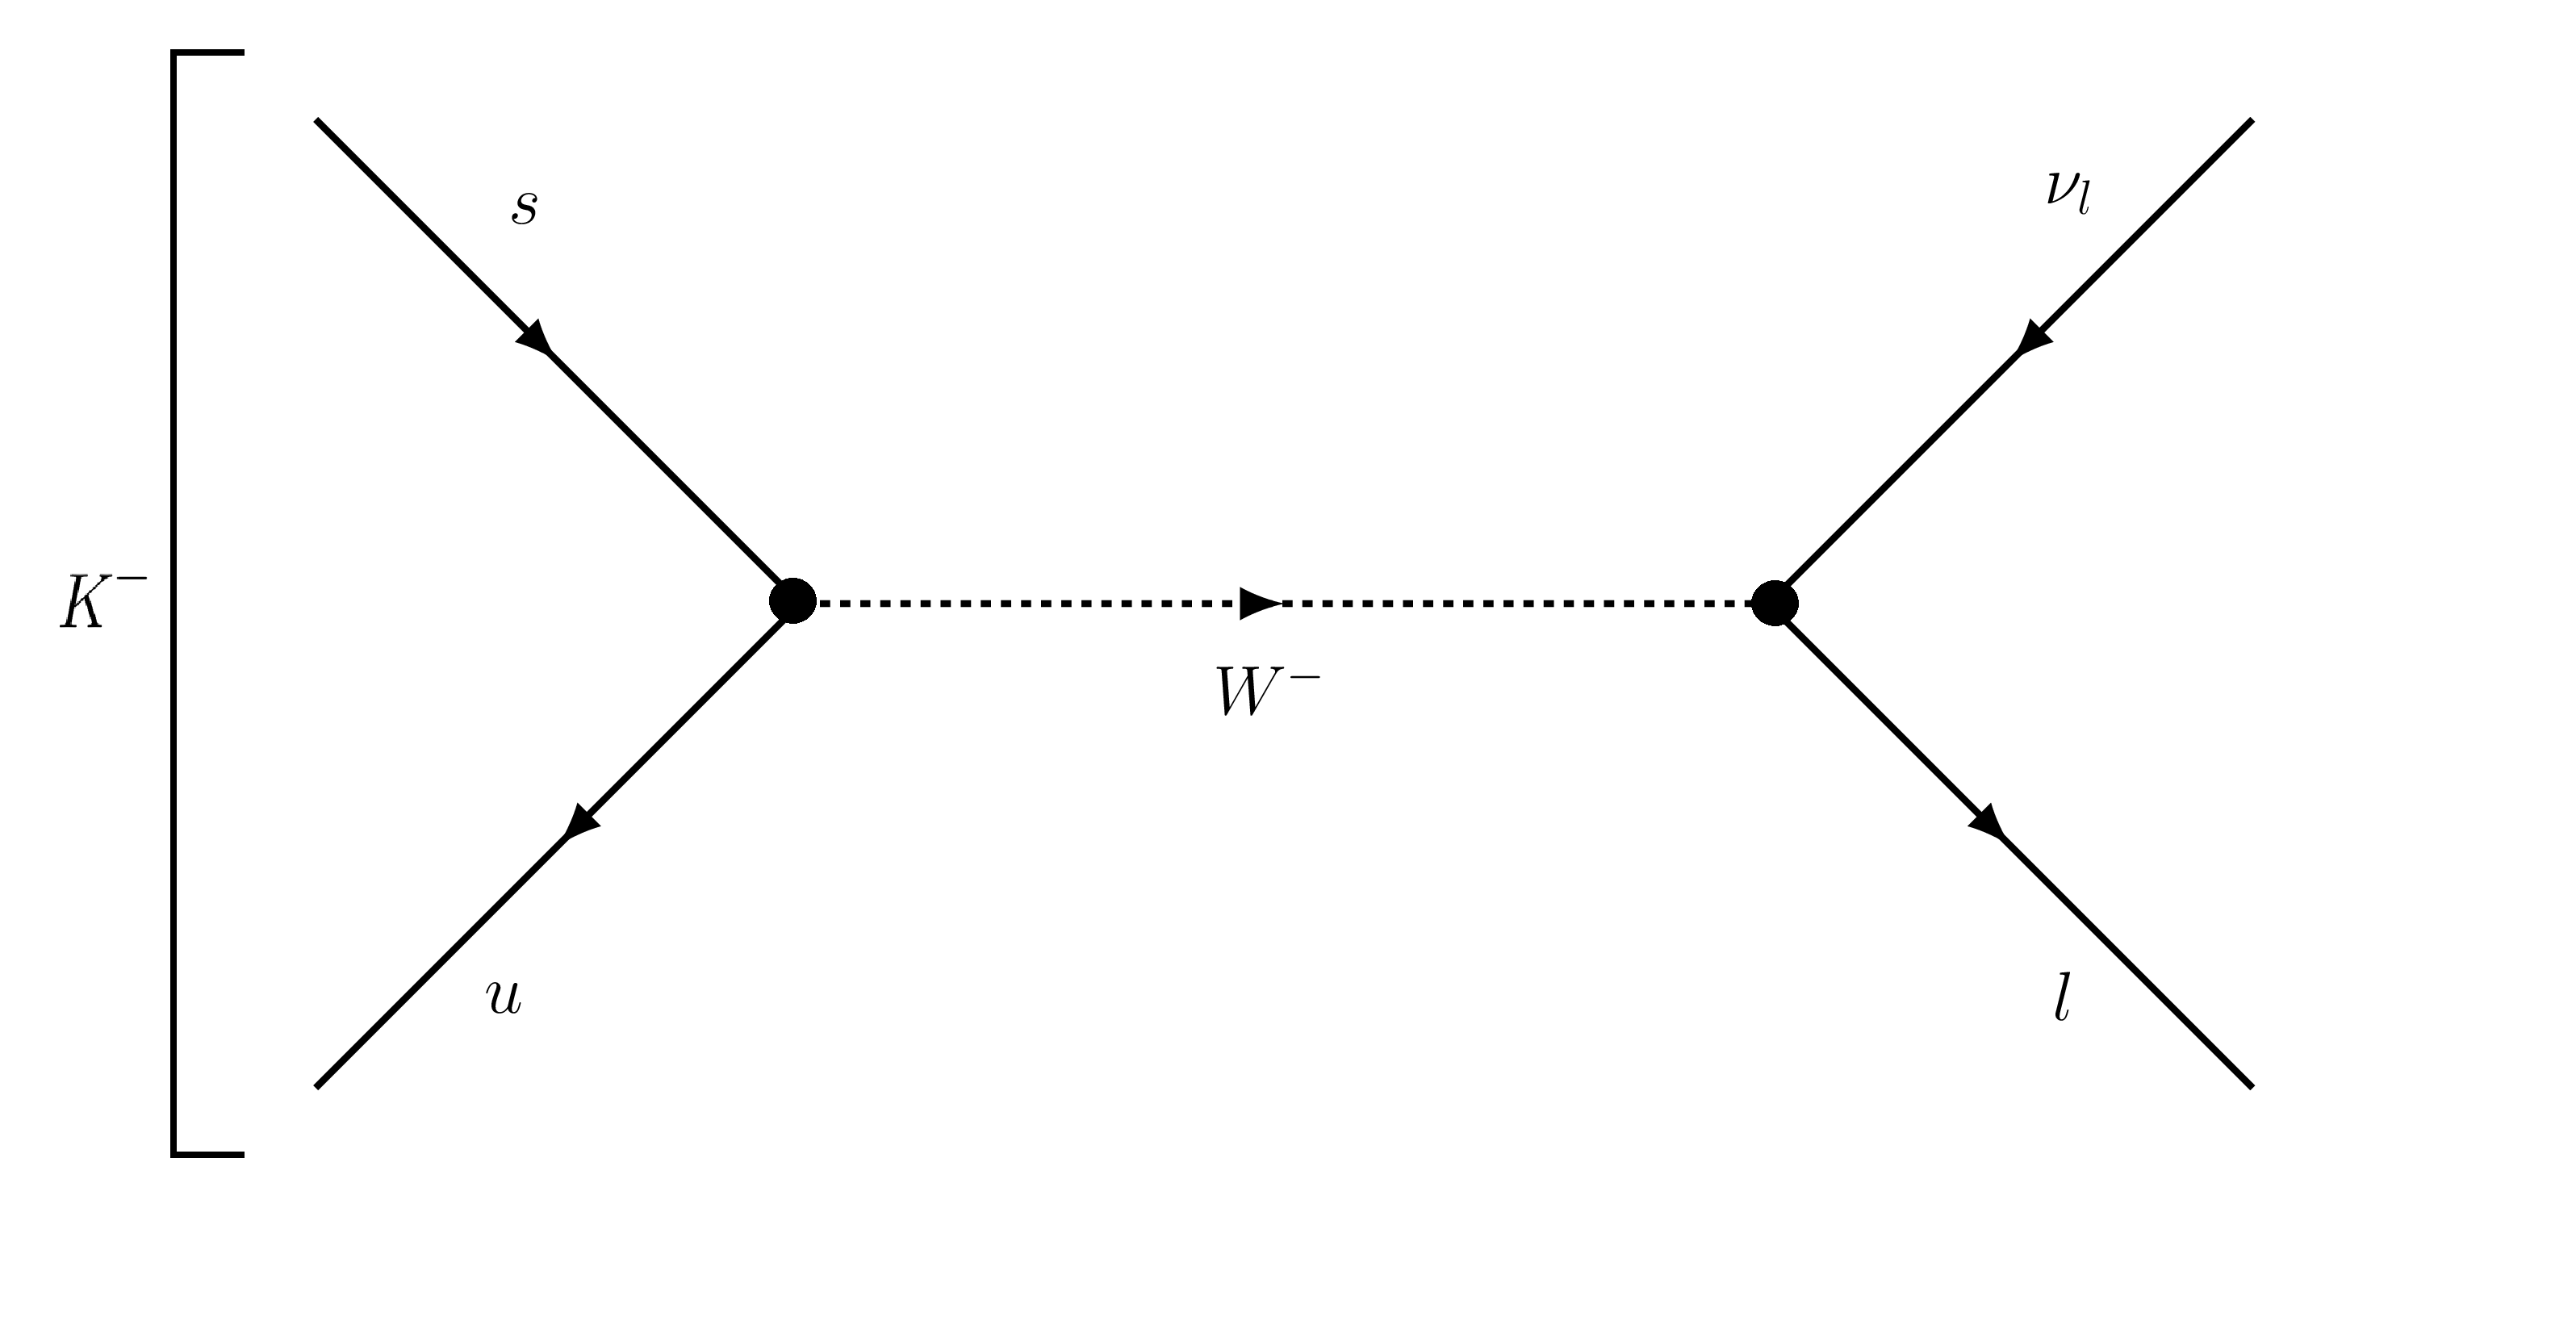
\includegraphics[width=0.95\textwidth]{C:/Users/Carmen/Desktop/Universidad/TFG/Borradores/img/kaon1.png}
	\caption[Diagrama de Feynman de quarks de $\PKm \rightarrow \Plm + \Pagnl$]
	{Diagrama de Feynman del modo leptónico de $\PKm$ en el Modelo de Quarks.}
	\label{fig:diagrama1}
\end{figure}

El vértice leptónico está totalmente definido a partir de las expresiones de corriente débil vistas en el formalismo anterior. Sin embargo, el vértice hadrónico es algo más complejo de explicar y puede hacerse mediante dos enfoques. El primero de ellos consiste en una descripción a partir de la composición de quarks de $\PKm$, pero este tratamiento presenta una dificultad de cálculo y formalismo teórico demasiado avanzado. Por ello, y dado que el mesón $\PK$ es una partícula de espín 0, resulta más sencillo describir dicho vértice hadrónico a partir de la ecuación de Klein-Gordon.

Siguiendo este segundo procedimiento, redibujamos el diagrama $\PKm \rightarrow \Plm + \Pagnl$ como se ve en la figura TAL. El punto gordo que se aprecia en el vértice hadrónico, simplemente indica que, como el mesón $\PKm$ posee una estructura interna más elemental, no sabemos de antemano cómo  interacciona con el propagador $\PWm$. Además, también se han etiquetado los momentos internos y externos de cada partícula que interviene.

\begin{figure}[ht!]
	\centering
	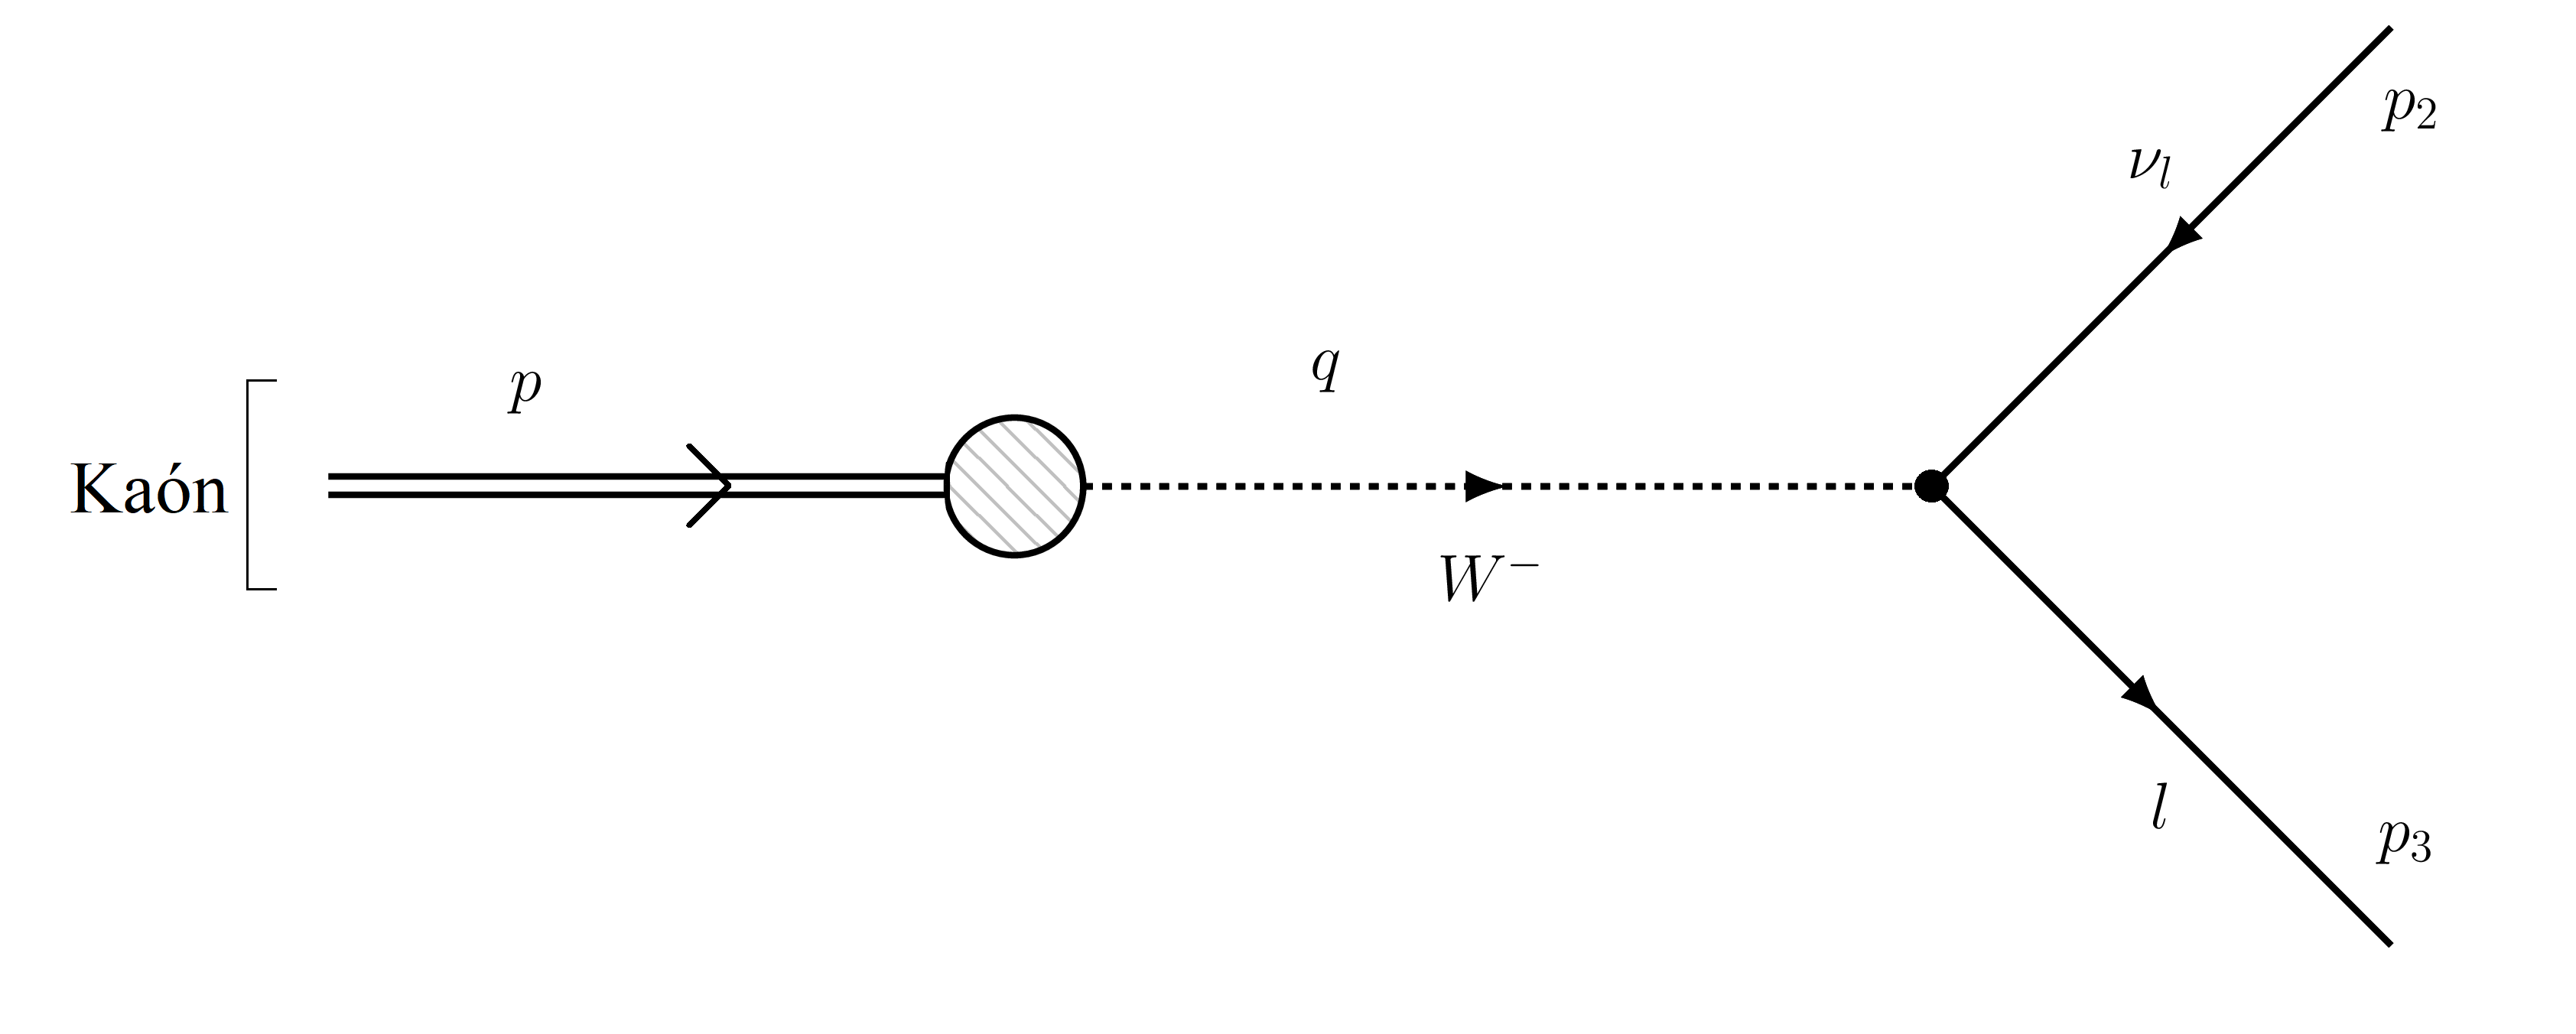
\includegraphics[width=0.95\textwidth]{C:/Users/Carmen/Desktop/Universidad/TFG/Borradores/img/kaon2.png}
	\caption[Diagrama de Feynman de $\PKm \rightarrow \Plm + \Pagnl$ con los momentos]
	{Diagrama de Feynman de $\PKm \rightarrow \Plm + \Pagnl$ con los momentos de cada partícula.}
	\label{fig:diagrama2}
\end{figure}

Analizamos el diagrama de la figura TAL y aplicamos las reglas de Feynman para calcular la amplitud de decaimiento del proceso, con el objetivo de hallar la probabilidad de que ocurran tales modos de decaimiento. 
